\chapter{Konzeption der Anwendung}\label{chapter_3}
Im vorigen Kapitel wurden die Anforderungen, sowie das Umfeld der Arbeit erläutert. In diesem Abschnitt wird der aktuelle Workflow beim Konfigurieren analysiert und anschließend an die mobile Umgebung angepasst. Nach der Workflow-Modellierung wird mit einer Entscheidung über den richtigen Typ der App.

\section{Aktueller Konfigurationsprozess}
Im aktuellen Prozess des Kunden wird ein Upgrade zuerst über den Produktkatalog gefunden. Im Katalog ist eine eindeutige Nummer enthalten, die bei der Bestellung verwendet wird. Die Fluggesellschaft nennt zu der Upgrade-Nummer, die Flugzeuge, die dieses Upgrade erhalten sollen. Diese Informationen werden von einem Design-Manager angenommen. Für die Weiterverarbeitung werden diese Informationen im Konfigurator-Client aus Abschnitt \ref{airbusConfigurator} erfasst. Die einzelnen Schritte der Erfassung sind in Abbildung \ref{webguiWorkflow} zu sehen. \par
\begin{figure}
\label{webguiWorkflow}
\centering
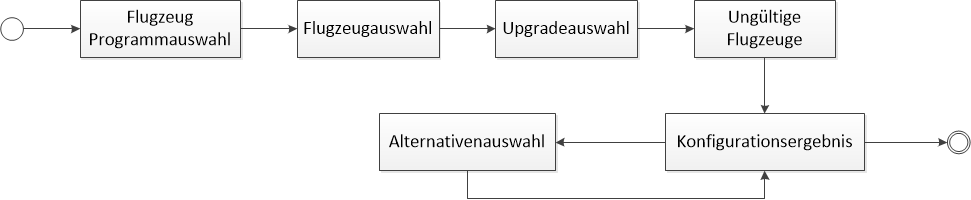
\includegraphics[width=300px]{images/workflow_webgui}
\caption{Programmablauf des Konfigurations-Clients}
\end{figure}
Im ersten Schritt wird das passende Flugzeugprogramm ausgewählt. Ein Programm ist eine grobe Einteilung für Flugzeuge nach deren Größe und Art. Die Auswahl ist eine erste Filterung der Datensätze. Des weiteren wird mit Hilfe des Programms das Regelwerk, welches auf dem Konfigurationsserver verwendet wird festgelegt. Anschließend folgt die Auswahl der entsprechenden Flugzeuge, welche ein Upgrade erhalten sollen. Die Auswahl kann nach bestimmten Kriterien gefiltert werden. Bei der Bestellung eines Upgrades wird die Flugzeugnummer angegeben, womit eine schnelle Auswahl erfolgen kann. Sind die Flugzeuge ausgewählt, werden Upgrades aus einer Liste selektiert. Es sind alle verfügbaren Updates aufgelistet. Die Auswahl erfolgt ebenfalls mit der eindeutigen Nummer, welche bei der Bestellung angegeben wurde. \par 

Nach der letzten Auswahl sind alle für die Konfiguration benötigten Elemente ausgewählt. Es folgt eine Validierung der Flugzeuge. Bei dieser Überprüfung werden die einzelnen Flugzeuge auf Konfigurationen untersucht, die in Widerspruch mit dem ausgewählten Upgrade stehen. Wenn keine Widersprüche gefunden wurden, ist die Bildung von sogenannten Konfigurationsgruppen die nächste Aufgabe. Eine Konfigurationsgruppe enthält Flugzeuge, die in die gleichen Zielzustände kommen, wenn das Upgrade eingebaut wird. Wenn es mehrere Möglichkeiten gibt, um in einen bestimmten Zustand des Flugzeuges zu kommen, werden sogenannte Alternativen in einer Konfigurationsgruppe enthalten. Damit die Konfiguration vollständig ist, muss der Anwender für die Gruppe eine Alternative auswählen. \par

Nachdem eine vollständige Konfiguration erzeugt wurde, wird daraus ein Excel-Dokument generiert. In diesem sind die Upgrades enthalten, die in den einzelnen Flugzeuge eingebaut werden müssen. Aus dem Dokument wird ein Upgrade-Angebot erstellt, dass anschließend dem Kunden vorgelegt wird.

\section{Workflow Modellierung}
Beim derzeitigen Konfigurationsprozess wird die eigentliche Konfiguration dem Experten überlassen. Ein Kunde wählt die Codes und Identifikationsnummern aus Katalog und derzeitigem Flugzeugbestand aus, erhält jedoch erst nach der Arbeit des Experten eine Bestätigung über die Gültigkeit der Konfiguration. Dieser Prozess wird bei der Portierung auf die mobile Umgebung verändert, so dass ein neuer Workflow entsteht. Die Prozesse sind im Folgenden in einen mobilen Konfigurationsprozess und den unterstützenden App-Workflow unterteilt.
\subsection{Mobiler Konfigurationsprozess}
Der derzeitige Workflow sollte die neuen Möglichkeiten einer mobilen Konfigurationsumgebung beinhalten. Mit der Mobilität ist ein Szenario einer direkten Konfiguration mit dem Kunden und einem Vertriebsexperten möglich. Beide können mithilfe der App direkt kommunizieren und das Ugrade gemeinsam durchführen. 
Primäres Ziel dieser Anpassung ist den Prozess kundenfreundlicher zu gestalten. Dieses Ziel soll durch folgende zwei Maßnahmen erreicht werden: \par

\begin{itemize}
        \item \textbf{Vereinfachung der Auswahl:} Das An- und Abwählen der Flugzeuge, bzw. der Upgrades soll vereinfacht werden. Die Auswahl soll nicht nur durch die Produktcodes, sondern durch verständlichere Weise erfolgen. 
        \item \textbf{Schnelleres Feedback:} Durch eine mobile Lösung soll bereits beim Kunden ein Feedback über die Gültigkeit der Konfiguration vorhanden sein.
\end{itemize}

Mit beiden Maßnahmen wird der Kunde stärker in den Prozess der Konfiguration einbezogen. Im Idealfall kann der Kunde die Anwendung alleine bedienen und der Experte steht nur Beratend zur Seite. Eine weitere Besonderheit der neuen Anwendung kann sein, dass der Kunde zu einem weiteren Upgrade bewogen wird, welches er erst beim Benutzen der Anwendung entdeckt. Eine weitere Möglichkeit ist das gezielte Anzeigen von kundenspezifische Informationen, die für weitere Kaufaktivitäten sorgen können. \par

\subsection{Workflow der App}
Der Anwendungsworkflow muss zu dem neuen fachlichen Prozess passen und ihn unterstützen. Dies geschieht durch Anpassungen an die Kommunikation mit dem Konfigurationsserver. 
Der aktuelle Client und der Server befinden sich auf der gleichen Umgebung. Somit können beide direkt miteinander kommunizieren und benötigen keine aufwändigen Webservice Schnittstellen. Für den neuen Prozess muss der Konfigurationsserver von der mobilen Umgebung erreichbar sein. Dies bedeutet, dass es eine Schnittstelle für die App geben muss. Die Kommunikation mit dem Webserver kann durch den mobilen Einsatz erschwert werden. Dies ist beispielsweise der Fall, wenn die Konfiguration beim Kunden vor Ort stattfindet und eine schlechte, bis gar keine Verbindung vorhanden ist. Aus diesem Grund ist bei den Nicht-Funktionalen Anforderung in Abschnitt \ref{non_functional_requirements} ein sogenannter Offline Modus enthalten, der die Zusammenstellung einer Konfiguration auch ohne Anbindung an den Konfigurator ermöglicht. Um eine flüssige Navigation gewährleisten zu können, muss die Kommunikation mit dem Server auf das Wesentliche konzentriert sein. Dies bedeutet, dass eine Konfiguration erst am Ende stattfindet und die einzelnen Schritte, die im derzeitigen Client durchgeführt werden zusammengelegt werden müssen. \par
\begin{figure}
\label{appWorkflow}
\centering
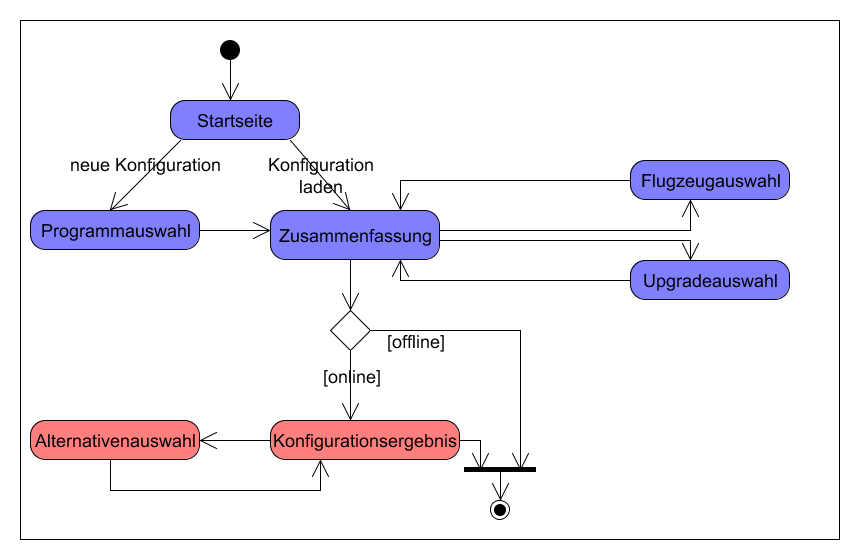
\includegraphics[width=400px]{images/workflow_app}
\caption{Programmablauf der Konfigurator-App}
\end{figure}
In Abbildung \ref{appWorkflow} ist der Anwendungsverlauf der App zu sehen. Analog zu der Weboberfläche wird bei einer neuen Konfiguration zuerst ein Programm (\textbf{Programmauswahl}) ausgewählt. Nach der Auswahl gelangt der Benutzer in eine \textbf{Zusammenfassung} der aktuellen Konfiguration. Von dieser Ansicht aus können Flugzeuge (\textbf{Flugzeugauswahl}) oder  Upgrades (\textbf{Upgradeauswahl}) selektiert werden. Sobald beides vorhanden ist, wird die Erreichbarkeit der Konfigurationsschnittstelle geprüft. Bei Verfügbarkeit befinden wir uns im "'Online"' Modus und es werden die Konfigurationsgruppen angezeigt. Nach erfolgter Konfiguration werden die Alternativen in einer separaten Ansicht (\textbf{Alternativenauswahl}) ausgewählt. Ist die Konfiguration vollständig, so kann das Upgrade direkt bestellt werden und den Update Vorgang beenden. Ist der Server nicht verfügbar, kann der Benutzer die aktuelle Konfiguration speichern und damit den Prozess abschließen. Anschließend kann die Auswahl direkt über den Startbildschirm geladen werden. \par

Um für einen möglichst geringen Kommunikationsaufwand mit dem Konfigurationsserver zu sorgen, wird der Server erst nach erfolgter Auswahl bedient. Der Typ bezieht sich auf eine Art Die Kommunikation wird alle zuvor beinhalteten Einzelschritte auf dem aktuellen Client zu einem Zusammenfügen. Die Trennung von Online (rot) und Offline (blau)  ist in der Abbildung ebenfalls aufgezeigt. 

\section{Auswahl der Anwendungsplattform}
Nachdem der Workflow, sowie die Anforderungen der Anwendung erläutert wurden, folgt in diesem Abschnitt die Auswahl der passenden Anwendungsplattform. Es werden die drei verschiedenen Anwendungstypen nativ, web und hybrid untersucht \cite{bib:mobilePlattform}. Bei jeder dieser Plattformen werden die bekanntesten Technologien verwendet. Die Untersuchung beruht auf den in Kapitel \ref{requirements} gestellten Anforderungen. Es werden folgende Auswahlkriterien verwendet:
\begin{itemize}
        \item \textbf{Offlinemodus:} Können offline Daten beliebig gespeichert werden? Gibt es eine passende Technologie für einen solchen Modus?
        
        \item \textbf{Sicherheit:} Da bei der Konfiguration sensible Daten verwendet werden, muss die Anwendung entsprechend gesichert werden können. Die einzelnen Sicherungsmaßnahmen sollen hierbei untersucht werden.
        
        \item \textbf{Schnittstelle:} Welche Möglichkeit für eine Schnittstelle zu dem Konfiguratorserver gibt es? 
        
        \item \textbf{Kundenpräferenz:} Gibt es eine bestimmte Technologie/Plattform, die vom Kunden explizit gewünscht ist? Hat die Technologie ein besonderes Alleinstellungsmerkmal?
        
        \item \textbf{Performance:} Für die Anzeige der einzelnen Produktbilder, sowie eine schnelle Navigation innerhalb der Anwendung ist die Performance des jeweiligen Typs wichtig.      
        
\end{itemize}
Bei der Auswahl der Technologien werden nur Plattformen ausgewählt, die auf Tabletgeräten verfügbar sind. Es werden alle Kriterien für den Anwendungstyp bewertet und zusätzlich für die einzelnen Technologien.


\subsection{Native Anwendungen}
Native Anwendungen sind auf die jeweilige Zielplattform beschränkt. Dieser Typ einer Anwendung beschränkt sich auf das zuvor gewählte Betriebssystem. Der geschriebene Programmcode kann meistens nur auf der Zielplattform verwendet werden. Für die Bewertung von nativen Anwendungen werden die drei am Meisten genutzten Betriebssysteme im Tabletbereich verwendet: Android, iOS und Windows 8\cite{bib:nativeBS}. \par

\textbf{Offlinemodus:} Bei einer nativen App ist keine Serveranbindung notwendig. Alle Daten können ohne eine Internetverbindung lokal auf dem Gerät selbst vorhanden sein. In einer nativen Anwendung können alle Dateioperationen, wie auf einem normalen Betriebssystem durchgeführt werden. Dies hat den großen Vorteil, dass auf den Speicher zugegriffen werden kann. Große Datensätze, die beim Offlinemodus anfallen, können damit auf dem Gerät gespeichert werden.  In diesem Kriterium ist das Verhalten für alle drei Betriebssysteme gleich, womit keine Unterscheidung der einzelnen Technologien notwendig ist.\par

\textbf{Sicherheit:} Durch die native Umgebung ist die Anwendung nur auf dem Betriebssystem vorhanden und in einer geschlossenen Umgebung. Die Kommunikation mit dem Webserver muss allerdings selbstständig verschlüsselt werden, insbesondere wenn Die Anwendung bei einem Kunden in dessen Netz verwendet wird. Ein weiteres Problem, welches native Anwendungen besitzen sind die lokalen Sicherheitslücken eines jedes Betriebssystems. Regelmäßig tauchen neue versteckte Fehler im Betriebssystem auf, die Schaden zufügen könnten. 

\begin{itemize}
        \item \textbf{Android und iOS:} Bei beiden Betriebssystemen werden regelmäßig Sicherheitslücken offengelegt. Die Angriffe auf beide Systeme ist zunehmend, wobei das iOS-System im Vergleich besser abschneidet und in mehreren 
        
        \item \textbf{Windows 8:} Durch die hohe Verbreitung von Windows Betriebssystemen sind diese Systeme besonders anfällig, bzw. oft verwendete Ziele bei Angriffen. Die breite Anzahl der Nutzer sorgt jedoch für ausreichend Lösungen zur Sicherung der Anwendung.
        
       
\end{itemize}

\textbf{Schnittstelle:} Für die Kommunikation mit dem Konfigurationsserver bieten sich bei einer nativen Anwendung Webservices an. Diese können in den Standards 
\subsection{Web Anwendungen}
phone gapp, gwt, 
\subsection{Hybride Anwendungen}
\subsection{Abwägung}
